\documentclass{article}
\usepackage{graphicx}
\usepackage[margin=1.5cm]{geometry}
\usepackage{amsmath}

\begin{document}
\twocolumn

\title{Monday warm-up: Kinematics III}
\author{Prof. Jordan C. Hanson}

\maketitle

\section{Memory Bank}

\begin{enumerate}
\item $g = 9.81$ m s$^{-2}$ ... The acceleration of gravity
\item $v_y(t) = a_y t + v_{i,y}$ (m/s)
\item $v_x(t) = a_x t + v_{i,x}$ (m/s)
\item $x(t) = \frac{1}{2}a_x t^2 + v_{i,x} t + x_{i}$ (m)
\item $y(t) = \frac{1}{2}a_y t^2 + v_{i,y} t + y_{i}$ (m)
\item $v_f^2 = v_i^2 + 2a\Delta x$ (m/s)$^2$.
\item $R = v_i^2 \sin(2\theta)/g$ ... Range formula.
\item $T = 2 v_i \sin(\theta)/g$ ... Time of flight formula.
\end{enumerate}

\section{Chapter 3 - Constant \\ Acceleration, and Projectile \\ Motion}

\begin{enumerate}
\item Consider Fig. \ref{fig:1}.  Suppose a soccer player must take a penalty kick from the outside corner of the penalty area towards the far goal post.  The distance to the goal line is 16.50 m, and the distance across the pitch is 11 m, plus 5.5 m, plus 7.32 m. (a) What is the straight-line distance from the ball to the far goal post? (b) Let the location of the ball be the origin.  If the goal post top corner is 2.45 m above the ground, where in 3D space is the goal post top corner? \\ \vspace{2.5cm}
\item When does the ball arrive at the goal, in the xy-plane? \\ \vspace{2cm}
\item How high above the pitch is the ball at that time?  Does the player score a goal? \\ \vspace{2cm}
\item Let's try to help the player score a goal.  (a) Write down (i) the formula for the motion in the xy-plane, involving speed, time, and displacement, and (ii) the formula for the motion in the vertical direction versus time. (b) Solve the former for time, and substitute it into the latter to eliminate the time variable.  You should have a quadratic equation for the vertical versus horizontal displacement of the ball. \\ \vspace{3cm}
\item Finally, keep the angle set to 30 degrees, and solve for the initial speed of the ball. With what initial speed should the ball be hit such that it scores the goal?
\end{enumerate}

\begin{figure}
\centering
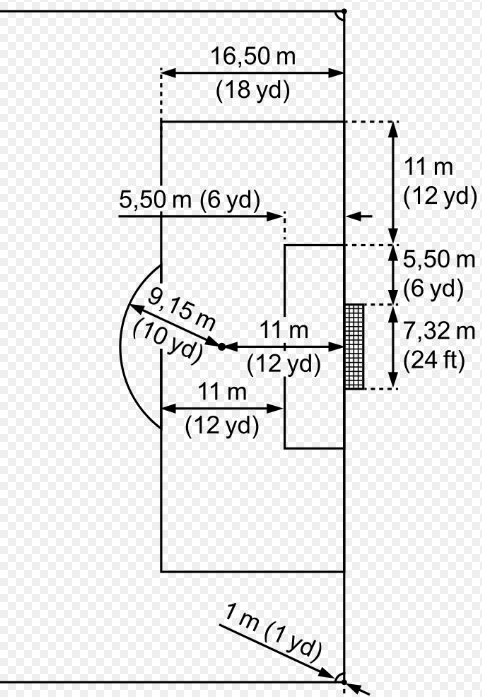
\includegraphics[width=0.25\textwidth]{figures/soccer_pitch.png}
\caption{\label{fig:1} A technical diagram of a football pitch.}
\end{figure}

\end{document}
